\documentclass[../main.tex]{subfiles}
\begin{document}
\chapter{Rigid Bodies}
Rigid body problems are a class of $N$-body problems where distances between the $N$ particles are fixed:
\[
  |\vec{x}_i - \vec{x}_j| = \text{constant}
\]
These are often tractable problems and usually arise due to very strong internal forces between particles.
Such a system of particles is known as a \textit{rigid body}.

The only motions a rigid body can experience are \textbf{translations of the centre of mass}, which we covered in \cref{systemsOfParticles}, and \textbf{rotations}, which we will cover now.
\section{Rotations}
\subsection{Angular Velocity}
In three dimensions, rotations are described by a vector quantity $\vec{\omega}$ called the \textit{angular velocity}.
\begin{definition}[Angular Velocity]
  The \textit{angular velocity} $\vec{\omega}$ is defined as:
  \[
    \vec{\omega} = \omega \uvec{n}
  \]
  where $\uvec{n}$ points along the axis of rotation and $\omega = |\vec{\omega}| = \dot{\theta}$ is the angular speed of rotation.
\end{definition}
\begin{remark}[Right Hand Rule]
  We define $\uvec{n}$ so that it always points in the direction where if you align you right hand thumb along the positive direction of the axis of rotation, the rotation is in the direction that your fingers curl.
\end{remark}
The key equation for rotations is:
\begin{equation}
  \dot{\vec{x}} = \vec{\omega} \times \vec{x} \label{angularVelocityCross}
\end{equation}
This can be seen in the following diagram:
\begin{center}
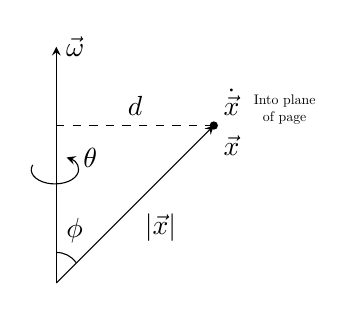
\begin{tikzpicture}[>=stealth]
  \draw[->] (0, 0)  -- (0, 3) node[right] {$\vec{\omega}$};
  \draw[->] (0, 0) -- (2, 2) node[below right] {$\vec{x}$} node[midway, below right] {$|\vec{x}|$};
  \fill (2, 2) circle (1.5pt) node[above right] {$\dot{\vec{x}}$};
  \node[text width=2cm, align=center, scale=0.5] at (2.9, 2.2) {Into plane of page};
  \draw[dashed] (2, 2) -- (0, 2) node[midway, above] {$d$};
  \draw[->, yscale=0.6] (-0.3,2.5) arc [start angle=-200,end angle=60,radius=0.3] node[xshift=0.3cm] {$\theta$};
  \draw (0.25,0.26) arc [start angle=35,end angle=90,radius=0.3] node[above right] {$\phi$};
\end{tikzpicture}
\end{center}
$\dot{\vec{x}}$ is orthogonal to both $\vec{\omega}$ and $\vec{x}$ and acts \textbf{into the plane of the page} in the above diagram.

The magnitude of $\uvec{n} \times \vec{x}$ is the distance between $\vec{x}$ and the axis of rotation:
\[
  |\uvec{n} \times \vec{x}| = |\uvec{n}||\vec{x}|\sin \phi = d
\]
and so:
\[
  |\dot{\vec{x}}| = \omega|\uvec{n} \times \vec{x}| = \omega d
\]
Therefore, the particle has speed $\omega d$, so $|\dot{\theta}| = \omega$

In addition to the angular velocity, a rotation must also specify a point about which the axis of rotation passes through.
For example, if we specify that the axis of rotation is the $z$-axis, then this does \textbf{not} specify the rotation as we do not know where the object is relative to this axis.
In the diagram, the vector $\vec{x}$ is measured from a point on the axis and we could have taken any point on the axis and it would be the same rotation.
The upshot of this is that in \cref{angularVelocityCross}, $\vec{x}$ must be relative to some arbitrary point on the axis of rotation.
\subsection{Moment of Inertia}
A particle rotating with angular velocity $\vec{\omega}$ has kinetic energy:
\begin{align*}
  T &= \frac{1}{2} m\dot{\vec{x}} \cdot \dot{\vec{x}} \\
    &= \frac{1}{2} m(\vec{\omega} \times \vec{x}) \cdot (\vec{\omega} \times \vec{x}) \\
    &= \frac{1}{2} m \omega^2 (\uvec{n} \times \vec{x}) \cdot (\uvec{n} \times \vec{x}) \\
    &= \frac{1}{2} m \omega^2 d^2
\end{align*}
where $d = |\uvec{n} \times \vec{x}|$ the perpendicular distance of $\vec{x}$ to the axis of rotation.

In a rigid body, all particles rotate with the same angular velocity $\vec{\omega}$, i.e.:
\[
  \dot{\vec{x}}_i = \vec{\omega} \times \vec{x}_i
\]
This ensures that the distances between particles remain fixed:
\begin{align*}
  \deriv{}{t}|\vec{x}_i - \vec{x}_j|^2 &= 2(\dot{\vec{x}}_i - \dot{\vec{x}}_j) \cdot (\vec{x}_i - \vec{x}_j) \\
                                       &= 2 [\vec{\omega} \times (\vec{x}_i - \vec{x}_j)] \cdot (\vec{x}_i - \vec{x}_j) \\
                                       &= 0
\end{align*}
and so $|\vec{x}_i - \vec{x}_j|$ is constant for all pairs of particles $i, j$ and so it remains a rigid body.
\begin{definition}[Moment of Inertia]
  For a particular choice of axis, the \textit{moment of inertia} $I$, of a rigid body is:
  \[
    I = \sum_{i = 1}^{N} m_i d^2_i
  \]
  where $d_i$ is the perpendicular distance of the $i$-th particle from the axis of rotation.
\end{definition}
The total kinetic energy of a rigid body is then:
\begin{align*}
  T &= \frac{1}{2} \sum_{i = 1}^{N} m_i \dot{\vec{x}}_i \cdot \dot{\vec{x}}_i \\
    &= \frac{1}{2} \omega^2 \sum_{i = 1}^{N} m_i d^2_i \\
    &= \frac{1}{2} I \omega^2
\end{align*}
\begin{remark}
  We see that $I$ is like the ``rotational mass'', the larger it is, the harder it is to rotate the rigid body.
\end{remark}

In a rigid body, the angular momentum is:
\begin{align*}
  \vec{L} &= \sum_{i = 1}^{N} m_i \vec{x}_i \times \dot{\vec{x}}_i \\
          &= \sum_{i = 1}^{N} m_i \vec{x}_i \times (\vec{\omega} \times \vec{x}_i)
\end{align*}
In this course, we will only consider the component of $\vec{L}$ along the axis of rotation $\uvec{n}$, i.e. $L = \vec{L} \cdot \uvec{n}$ so:
\begin{align*}
  L &= \omega \left(\sum_{i = 1}^{N} m_i \vec{x}_i \times (\uvec{n} \times \vec{x}_i)\right) \cdot \uvec{n} \\
    &= \omega \sum_{i = 1}^{N} m_i (\vec{x}_i \times (\uvec{n} \times \vec{x}_i)) \cdot \uvec{n} \\
    &= \omega \sum_{i = 1}^{N} m_i (\uvec{n} \times \vec{x}_i) \cdot (\uvec{n} \times \vec{x}_i) \text{ as $(\vec{a} \times \vec{b}) \cdot \vec{c} = (\vec{c} \times \vec{a}) \cdot \vec{b}$} \\
    &= \omega \sum_{i = 1}^{N} m_i d^2_i \\
    &= \omega I
\end{align*}
\begin{remark}
  Linear momentum is velocity times mass and here angular momentum along the axis is angular velocity times moment of inertia, so again in the moment of inertia acts like a ``rotational mass''.
\end{remark}
Recall from \cref{totalAngularMomentum}, that external the \textit{torque} $\vec{G}$ changes angular momentum, that is, $\dot{\vec{L}} = \vec{G}$.
If the torque is along the axis of rotation, then $\vec{G} = G\uvec{n}$ for some scalar $G$.
If we dot both sides of $\dot{\vec{L}} = \vec{G}$  to compare components along the axis, we have:
\[
  \dot{\vec{L}} \cdot \uvec{n} = \vec{G} \cdot \uvec{n} \implies \dot{L} = G \implies \dot{\omega}I = G
\]
\begin{remark}[Note]
  So far, all of this depends on the axis of rotation that we choose and is not an intrinsic property of the body.

  In Part II, we will define a more invariant \textit{inertia tensor} that packages up all the information needed to find the moment of inertia of a rigid body about \textbf{any axis}.
\end{remark}
\subsection{Computing Moment of Inertia}
\subsubsection{Approximating Sums with Integrals}
The calculate the moment of inertia, we can utilise that for large $N$, the particles are densely spaced and so we can approximate the unwieldy sums using integrals.

For any function $f(\vec{x})$:
\[
  \sum_{i = 1}^{N} m_i f(\vec{x}_i) \approx \int \rho(\vec{x}) f(\vec{x}) \d^3{\vec{x}}
\]
where $\rho$ is the \textit{density} of the rigid body at $\vec{x}$, although we typically consider situations with uniform density, i.e. $\rho(\vec{x}) = \rho_0\ \forall x \in \R^3$.

If we want the mass of the body $M$, we set $f(\vec{x}) = 1$ and so:
\[
  M = \int \rho(\vec{x}) \d^3{\vec{x}}
\]
Similarly, for the moment of inertia, we set $f(\vec{x}) = x^2_{\perp}$ where $x_{\perp}$ is the perpendicular distance of $\vec{x}$ from the axis of rotation, and so:
\[
  I = \int \rho(\vec{x}) x^2_\perp \d^3{\vec{x}}
\]
\begin{example}[Moments of Inertia for Basic Shapes]
  Consider the following rigid bodies with a constant density $\rho$.
  \begin{enumerate}
    \item Consider a 1D ring $R$ of radius $a$:
      \begin{center}
      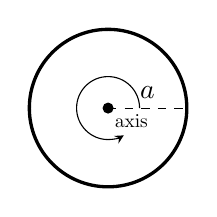
\begin{tikzpicture}[>=stealth]
        \draw[very thick] (0, 0) circle (1);
        \draw[dashed] (0, 0) -- (1, 0) node[midway, above] {$a$};
        \fill (0, 0) circle (2pt) node[below right, scale=0.7] {axis};
        \draw[->] (0.4, 0) arc [start angle=0,end angle=300,radius=0.4];
      \end{tikzpicture}
      \end{center}
      Its mass is:
      \[
        M = 2\pi a \rho
      \]
      and if it is rotating through its centre the moment of inertia is:
      \[
        I = \int_{R} \rho a^2 \d{\vec{x}} = 2\pi \rho a^3
      \]
      as the length of $R$ is $2 \pi a$.
      We can then relate the two by $I = Ma^2$.
    \item Consider a 1D rod of length $\ell$:
      \begin{center}
      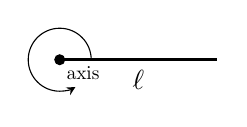
\begin{tikzpicture}[>=stealth]
        \draw[very thick] (0, 0) -- (2, 0) node[midway, below] {$\ell$};
        \fill (0, 0) circle (2pt) node[below right, scale=0.7] {axis};
        \draw[->] (0.4, 0) arc [start angle=0,end angle=300,radius=0.4];
      \end{tikzpicture}
      \end{center}
      Its mass is:
      \[
        M = \ell \rho
      \]
      and if it is rotating about one of its ends, the moment of inertia is:
      \[
        I = \rho \int_{0}^{\ell} x^2 \d{x} = \frac{\rho \ell^3}{3} = \frac{1}{3}M\ell^2
      \]
    \item Consider a 2D disc $D$ of radius $a$:
      \begin{center}
      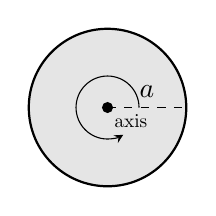
\begin{tikzpicture}[>=stealth]
        \filldraw[fill=gray!20, draw=black, thick] (0, 0) circle (1);
        \draw[dashed] (0, 0) -- (1, 0) node[midway, above] {$a$};
        \fill (0, 0) circle (2pt) node[below right, scale=0.7] {axis};
        \draw[->] (0.4, 0) arc [start angle=0,end angle=300,radius=0.4];
      \end{tikzpicture}
      \end{center}
      Its mass is:
      \[
        M = \pi a^2 \rho
      \]
      and if it is rotating through its centre, the moment of inertia is:
      \[
        I = \int_{D} \rho x^2_\perp \d^2{\vec{x}}
      \]
      Using methods from Vector Calculus, we change to plane polar coordinates on the disc.
      We have $x_{\perp} = r$ and we introduce the Jacobian $|J| = r$ so:
      \begin{align*}
        I &= \int_{0}^{2\pi} \int_{0}^{a} \rho r^2 \cdot r\d{r} \d{\theta} \\
          &= \rho \int_{0}^{2\pi} \d{\pi} \int_{0}^{a} r^3 \d{r} \\
          &= \frac{\pi}{2}\rho a^4 = \frac{1}{2}Ma^2
      \end{align*}
    \item For a 3D sphere $V$ of radius $a$, its mass is $M = \frac{4}{3} \pi a^3 \rho$ and if it is rotating about an axis through its centre, the moment of inertia is:
      \[
        I = \int_{V} \rho x^2_\perp \d^3{\vec{x}}
      \]
      Using methods from Vector Calculus, we change to spherical coordinates using the axis of rotation as the $z$-axis.
      We have $x_{\perp} = r \sin \theta$ and we introduce the Jacobian $|J| = r^2 \sin \theta$ so:
      \begin{align*}
        I &= \int_{0}^{2\pi} \int_{0}^{\pi} \int_{0}^{a} \rho(r \sin \theta)^2 \cdot r^2 \sin \theta \d{r} \d{\theta} \d{\phi} \\
          &= \rho\int_{0}^{2\pi} \d{\phi} \int_{0}^{\pi} \sin^3 \theta \d{\theta} \int_{0}^{a} r^4 \d{r} \\
          &= \rho \cdot 2 \pi \cdot \frac{4}{3} \cdot \frac{a^5}{5} \\
          &= \frac{8\pi}{15} \rho a^5 = \frac{2}{5}Ma^2
      \end{align*}
  \end{enumerate}
\end{example}
\begin{remark}
  In these examples, we see that if the shape of the rigid body is defined by a single length $a$, then $I = kMa^2$ where $k$ is some constant.
\end{remark}
\subsubsection{Perpendicular Axis Theorem}
\begin{lemma}[Perpendicular Axis Theorem]
  For a 2D rigid body, sometimes called a \textit{lamina}, on the $(x, y)$-plane, its moments of inertia $I_x$, $I_y$, and $I_z$ about the $x$, $y$ and $z$ axes respectively are:
  \begin{align*}
    I_x &= \int \rho(\vec{x}) \cdot y^2 \d^2{\vec{x}} \\
    I_y &= \int \rho(\vec{x}) \cdot x^2 \d^2{\vec{x}} \\
    I_z &= \int \rho(\vec{x}) \cdot (x^2 + y^2) \d^2{\vec{x}} = I_x + I_y
  \end{align*}
\end{lemma}
\begin{proof}
  If we take the $x$-axis to be the axis of rotation, then the perpendicular distance of a particle at $(x, y)$ to the axis is just $y$ and so:
  \[
    I_x = \int \rho(\vec{x}) \cdot y^2 \d^2{\vec{x}}
  \]
  and similarly about the $y$ axis.

  If we take the $z$-axis to be the axis of rotation, then the perpendicular distance of a particle at $(x, y)$ to the axis is just its distance from the origin and so:
  \[
    I_z = \int \rho(\vec{x}) \cdot \left(\sqrt{x^2 + y^2}\right)^2 \d^2{\vec{x}} = \int \rho(\vec{x}) \cdot (x^2 + y^2) \d^3{\vec{x}} = I_x + I_y
  \]
\end{proof}
\subsubsection{Parallel Axis Theorem}
\begin{lemma}[Parallel Axis Theorem]
  If we know the moment of inertia of a 3D rigid body about some axis through the CoM, then the moment of inertia $I_{\text{para}}$ about any other axis parallel to that axis is given by:
  \[
    I_{\text{para}} = I_{\text{CoM}} + Mh^2
  \]
  where $h$ is the distance between the two axes.
\end{lemma}
\begin{remark}
  Since $h^2 \geq 0$, $I_{\text{para}} \geq I_{\text{CoM}}$.
  This means that the moment of inertia for a given axis direction is minimised when the axis passes through the CoM.
\end{remark}
\begin{proof}
  Recall from \cref{relativeSum}, that if we write $\vec{x}_i = \vec{R} + \vec{y}_i$, then:
  \[
    \sum_{i = 1}^{N} m_i \vec{y}_i = \vec{0}
  \]
  By definition, the moment of inertia is:
  \[
    I = \sum_{i = 1}^{N} m_i (\uvec{n} \times \vec{x}_i) \cdot (\uvec{n} \times \vec{x}_i)
  \]
  Continued next lecture.
\end{proof}
\end{document}
